\documentclass[12pt]{article}

\usepackage[margin=1.0in]{geometry}
\usepackage{graphicx}
\usepackage{listings}
\usepackage{tabto}
\usepackage{multicol}
\usepackage{lipsum}
\usepackage{caption}
\usepackage{mwe}
\usepackage{tikz}
\usepackage{tabto}
\usetikzlibrary{automata,positioning}
\usepackage{enumitem}
\usepackage{amsmath}
\usepackage{amssymb}
\graphicspath{ {./} }


\begin{document}

\title{CS4347 : Database Systems\\Homework Assignment 6}
\author{Matthew McMillianmgm160130@utdallas.edu}
\maketitle



\begin{enumerate}

	\item  Add the operation commit at the end of each of the transactions T1 and T2 in Figure 20.2, and then list all possible schedules for the modified transactions. Determine which of the schedules are recoverable, which are cascadeless, and which are strict. \\ \\
	

 	\begin{center}
 		Recoverable Schedules
 	\end{center}
    \begin{minipage}{.5\linewidth}

      \centering
       \begin{tabular}{|l|l|}
\hline
T1 & T2 \\ \hline
read\_item(x) &  \\ \hline
x := x - n &  \\ \hline
write\_item(x) &  \\ \hline
read\_item(y) &  \\ \hline
y := y + n &  \\ \hline
write\_item(y) &  \\ \hline
commit; &  \\ \hline
 & read\_item(x) \\ \hline
 & x := x + m \\ \hline
 & write\_item(x) \\ \hline
 & commit; \\ \hline
\end{tabular}
    \end{minipage}%
    \begin{minipage}{.5\linewidth}
      \centering
      
        \begin{tabular}{|l|l|}
\hline
T1 & T2 \\ \hline
read\_item(x) &  \\ \hline
x := x - n &  \\ \hline
write\_item(x) &  \\ \hline
read\_item(y) &  \\ \hline
 & read\_item(x) \\ \hline
y := y + n &  \\ \hline
write\_item(y) &  \\ \hline
commit; &  \\ \hline
 & x := x + m \\ \hline
 & write\_item(x) \\ \hline
 & commit; \\ \hline
\end{tabular}
    \end{minipage} 

	
	\pagebreak
\begin{center}
 		Cascadless Schedules
 \end{center}
    \begin{minipage}{.5\linewidth}
  
      \centering
       \begin{tabular}{|l|l|}
\hline
T1 & T2 \\ \hline
read\_item(x) &  \\ \hline
x := x - n &  \\ \hline
write\_item(x) &  \\ \hline
read\_item(y) &  \\ \hline
y := y + n &  \\ \hline
write\_item(y) &  \\ \hline
commit; &  \\ \hline
 & read\_item(x) \\ \hline
 & x := x + m \\ \hline
 & write\_item(x) \\ \hline
 & commit; \\ \hline
\end{tabular}
    \end{minipage}%
    \begin{minipage}{.5\linewidth}
      \centering

\begin{tabular}{|l|l|}
\hline
T1 & T2 \\ \hline
 & read\_item(x) \\ \hline
 & x := x + m \\ \hline
 & write\_item(x) \\ \hline
 & commit; \\ \hline
read\_item(x) &  \\ \hline
x := x - n &  \\ \hline
write\_item(x) &  \\ \hline
read\_item(y) &  \\ \hline
y := y + n &  \\ \hline
write\_item(y) &  \\ \hline
commit; &  \\ \hline
\end{tabular}
    \end{minipage} 


\begin{center}
 		Strict Schedules
 \end{center}
    \begin{minipage}{.5\linewidth}
  
      \centering
       \begin{tabular}{|l|l|}
\hline
T1 & T2 \\ \hline
read\_item(x) &  \\ \hline
x := x - n &  \\ \hline
write\_item(x) &  \\ \hline
read\_item(y) &  \\ \hline
y := y + n &  \\ \hline
write\_item(y) &  \\ \hline
commit; &  \\ \hline
 & read\_item(x) \\ \hline
 & x := x + m \\ \hline
 & write\_item(x) \\ \hline
 & commit; \\ \hline
\end{tabular}
    \end{minipage}%
    \begin{minipage}{.5\linewidth}
      \centering

\begin{tabular}{|l|l|}
\hline
T1 & T2 \\ \hline
 & read\_item(x) \\ \hline
 & x := x + m \\ \hline
 & write\_item(x) \\ \hline
 & commit; \\ \hline
read\_item(x) &  \\ \hline
x := x - n &  \\ \hline
write\_item(x) &  \\ \hline
read\_item(y) &  \\ \hline
y := y + n &  \\ \hline
write\_item(y) &  \\ \hline
commit; &  \\ \hline
\end{tabular}
    \end{minipage} 
\\ \\ \\
Interestingly enough, for this example we can use the same cascading schedule to define our strict schedule. We could vary if it we had a commit before the read$\_$item(y) part. \\ 

	\item  List all possible schedules for transactions T1 and T2 in Figure 20.2, and determine which are conflict serializable (correct) and which are not. \\ \\
	In the schedules listed above, the cascading and strict schedules are conflict equivalent. The recoverable schedules are conflict equivalent to themselves, however in general the recoverable and cascadeless solutions are not conflict equivalent to the recoverable schedules.
	\pagebreak
	\item Consider the three transactions T1, T2, and T3, and the schedules S1 and S2 given below. Draw the serializability (precedence) graphs for S1 and S2, and state whether each schedule is serializable or not. If a schedule is serializable, write down the equivalent serial schedule(s). \\ 
	
	\begin{center}
 		Precedence Graphs for S1 and S2 \\
 \end{center}
    \begin{minipage}{.5\linewidth}
  
      \centering
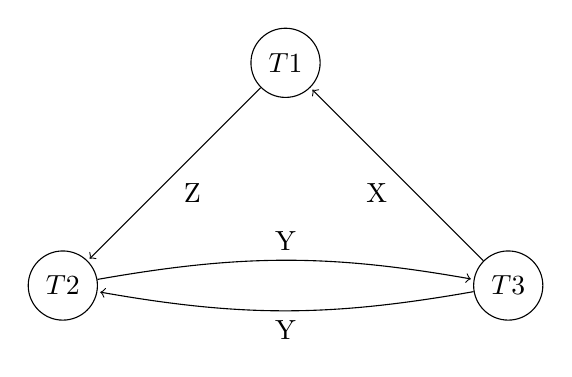
\begin{tikzpicture}[shorten >=1pt,node distance=4cm,on grid,auto] 
   \node[state] (T1)   {$T1$}; 
   \node[state] (T2) [below left=of T1] {$T2$}; 
   \node[state] (T3) [below right=of T1] {$T3$}; 
    \path[->] 
    (T1) edge  node {Z} (T2)
    (T2) edge [bend left=10, above] node {Y} (T3)          
    (T3) edge [bend left=10, below]  node {Y} (T2) 
          edge node {X} (T1);
\end{tikzpicture}
    \end{minipage}%
    \begin{minipage}{.5\linewidth}
      \centering


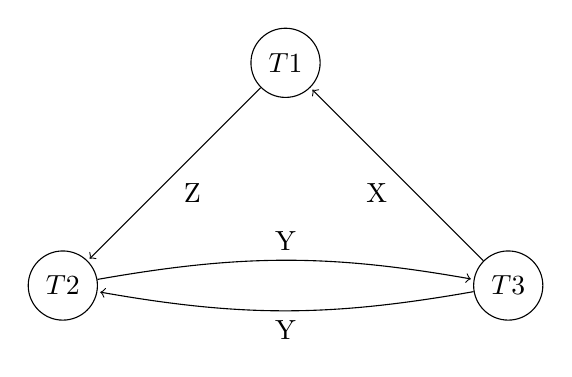
\begin{tikzpicture}[shorten >=1pt,node distance=4cm,on grid,auto] 
   \node[state] (T1)   {$T1$}; 
   \node[state] (T2) [below left=of T1] {$T2$}; 
   \node[state] (T3) [below right=of T1] {$T3$}; 
    \path[->] 
    (T1) edge  node {Z} (T2)
    (T2) edge [bend left=10, above] node {Y} (T3)          
    (T3) edge [bend left=10, below]  node {Y} (T2) 
          edge node {X} (T1);
\end{tikzpicture}
    \end{minipage} 
\\ \\ \\
Both of the precedence graphs are the same. We can conclude that since there is a cycle between two nodes that neither processes are serializable. \\
	

	\item  Consider schedules S3, S4, and S5 below. Determine whether each schedule is strict, cascadeless, recoverable, or nonrecoverable. (Determine the strictest recoverability condition that each schedule satisfies.)
	\begin{itemize}
		\item A recoverable schedule is one where if a transaction reads an item previously written by another transaction, the commit operation must occur for the first transaction first. This is true of the first sequence. w3(y) happens before r2(y), however T3 commits before T2 so this makes this a recoverable solution.
		\item This is a non-recoverable schedule. It is not cascadeless since no items are read only after committed transactions, items do not follow a strict schedule since a commit doesn't occur before other reads,, and it is not recoverable since nothing reads after write operations.
			\item This is a non-recoverable schedule. It is not cascadeless since no items are read only after committed transactions, items do not follow a strict schedule since a commit doesn't occur before other reads, and it is not recoverable since nothing reads after write operations.
	\end{itemize}

	

\end{enumerate}


\end{document}
